\documentclass[titlepage]{article}
\usepackage[utf8]{inputenc}
\usepackage{setspace}
\usepackage{lineno}
\usepackage[margin=0.5in]{geometry}
\usepackage{csvsimple}
\usepackage{graphicx}
\usepackage{caption}
\usepackage{subcaption}
\usepackage{float}
\usepackage{gensymb}
\restylefloat{table}
\linenumbers
\doublespacing

\title{CMEE Miniproject: Population Growth \\ 
\large How well do different mathematical models, e.g., based upon population growth (mechanistic) theory vs. phenomenological ones, fit to functional responses data across species?}
\author{Amy Bo Tinky Solman\\
Imperial College London}
\date{6th March 2020\\
Word count: 3088}

\begin{document}

\maketitle

\begin{abstract}
    \centering
    This investigation was conducted to assess the goodness of fit of the Logistic, Gompertz, Baranyi, Buchanan, Polynomial, Quadratic and Linear models in bacterial growth curves. The data was collated from 11 studies from around the world. These amounted to 285 individual growth curves. The goodness of fit of each model was assessed by finding the coefficient of determination ($R^2$), Akaike's information criteria (AIC) and Bayesian information criterion (BIC). All models except the Linear model had a mean $R^2$ value of 0.85 or higher, showing that all but the Linear model performed well in describing the data. Based on the AIC and BIC values, the Logistic model was determined to be the best fitting model across all datasets and most species groups, as well as being particularly successful for predicting datasets with higher temperature treatments. These findings support previous research that indicates the Logistic model is effective in predicting bacterial growth curves, whilst requiring less parameter inputs than competing models.
\end{abstract}

\section{Introduction}

The study of population dynamics began in earnest in the early 20th century to manage and predict agricultural stocks in the wake of the World Wars \cite{KingslandSharonE1995Mn:e}. Since that time the field has developed and been applied to conservation efforts and in predicting the impacts of climate change \cite{ozgul2010coupled} \cite{hunter2010climate}. Fluctuations in population abundance can impact keystone processes and ecosystem dynamics \cite{sinclair2003mammal}. Emergent functional characteristics such as disease transmission can also be affected by host/pathogen population dynamics \cite{alexander1996population}. Moreover, population dynamics for species such as phytoplankton dictates rates of carbon fixation in aquatic systems \cite{reynolds2000regulation}.\ 

\indent Turchin asserts that there are three general laws of population dynamics: populations tend to grow exponentially, population growth is self-limiting and consumer-resource populations tend to oscillate \cite{TurchinPeter2001Dpeh}. Patterns of population dynamics include exponential growth, logistic growth and predator-prey interactions \cite{RockwoodLarryL.2015ItPE}. Exponential population growth describes a continually increasing number of individuals under conditions where resources are not limiting \cite{BotsfordLouisW.author2019Pdfc}. Logistic growth occurs when population growth rate decreases as it reaches carrying capacity \cite{KingslandSharon1982TRMT}. Predator-prey interactions are concerned with the feeding relationship between species, resulting in a temporally staggered undulating pattern, with predator numbers lagging behind prey \cite{BerrymanAlanA.AlanAndrew1937-2008Ps:a}.  \

\indent  Population ecologists are concerned with quantifying these patterns of growth. Levin's states that, "it is of course desirable to work with manageable models that maximise generality, realism and precision" \cite{levins1966strategy}. Over the past century a wealth of models have been devised to fit the various patterns of population growth observed in nature. Models may be either phenomenological or mechanistic. Mechanistic models often need a large number of parameters to describe complex ecological systems, whilst phenomenological models may need relatively few \cite{transtrum2016bridging}. In mechanistic models then we loose generality, in gaining precision and realism. In phenomenological models we may loose sight of the real-world mechanisms at play.\

\indent Understanding microbial patterns of population growth is important for food microbiology, risk assessment and water protection \cite{zwietering1990modeling} \cite{nauta2002modelling} \cite{dukan1996dynamic}. Microbial growth patterns also play a significant role in ecosystem processes, particularly in habitats newly exposed through climate change \cite{bradley2017microbial}. Typically, bacteria in culture has a four phase growth curve: the lag phase, exponential or log phase, stationary and death phase \cite{al2008studying}. Three types of models can be applied to bacterial growth: 1) Primary models concerning changes in population over time; 2) Secondary models predicting changes in population in changing environmental conditions; 3) Tertiary models combining the two \cite{whiting1995microbial}\cite{grijspeerdt1999estimating}. The models presented in this report will deal only with bacterial communities during the first three growth phases. \

\indent  This investigation compares a variety of both mechanistic and phenomenological mathematical Primary models, to see how well each characterises patterns of bacterial growth over time. Here I use a variety of statistical measures to find which model best fits the bacterial sigmoid growth curves see in the given data set.

\section{Data}
The dataset used in this report, LogisticGrowthData.csv, is a amalgamation of 11 reports, detailing 285 unique bacterial growth curves, over 17 temperature conditions and 19 mediums. 46 species or strain of bacteria are documented.

\section{Methods}

\subsection{Computing Tools}
The original data set was prepared for non-linear least squares model fitting through a Python script (data\_prep.py). I used the pandas software library to import the csv file. I then isolated single growth curves by combining Citation, Species and Temperature values and assigning these to a new column. The pandas factorize function was called to apply numerical values to this new column, thus attaching growth curve 'IDs' to each row of data. Finally, the modified data was saved to a new csv file (modified\_data.csv). pandas was employed here as it is a powerful and popular tool for data manipulation, allowing for easy importation, modification and exportation of this large csv file.

The modified dataset was imported into R (NLLSfittingscript.R). minpack.lm and plyr packages were imported. minpack.lm allows R to interface with the Levenberg-Marquardt Nonlinear Least-Squares algorithm. The standard function calls the Gauss-Newton algorithm, which is less robust. When this script was run without importing minpack.lm, four of the seven models failed to fit any growth curves, with only polynomial, quadratic and linear fits being successful. After importing minpack.lm, all models were fit to the data with some degree of success. plyr is a commonly used data manipulation tool. The package was used to merge the statistics and plots lists of data frames, into a two single data frames ready to be exported. 

The modified data, statistical results and plot results were then imported into a second R script (plot\_analysis.R). For this script I imported ggplot2, plyr and dplyr. ggplot2 is a powerful graphics package, specifically designed for creating plots. Here I used ggplot2 to plot each growth curve with any successful model fits. Each plot was then exported as an individual pdf to the plots sub-directory. plyr was used to merge the list of final\_stats data frames, into a single data frame (merged\_data). dplyr was used to calculate the total number of times each model was the best fit to a growth curve using a measure of $R^2$, AIC or BIC. The total number of best fits of each model was then added to the total data frame as an additional column.  

Finally, two bash scripts were used. The first, CompileLaTex.sh was used to compile my LaTex FinalReport.tex document, along with bibliography.bib. The second bash script run\_Miniproject.sh, called data\_prep.py, NLLSfittingscript.R, plot\_analysis.R and CompileLaTex.sh, to execute the entire project, beginning with the original data set and ending with this FinalReport document. No additional packages were used within either bash script.


\subsection{Models}
Below is a brief description of each model used in this project, and the reason for its selection. Most sigmoidal growth models used between three and four adjustable parameters \cite{peleg2011microbial}. Each of the first four models used calculated starting values for initial cell culture density, maximum cell culture density and maximum growth rate. The Gompertz, Baranyi and Buchanan models also used a starting value for the duration of the lag phase.
  Starting values were obtained by running a linear model on the logarithmic population and time of each data set. The coefficients of this linear model were stored. The time values were reduced by 5\% and the linear model re-run until the time had been reduced to 10\%. The coefficients of the final, reduced linear model were used to calculate the r\_max\_start (maximum growth rate) and t\_lag\_start (lag phase) values. N\_0\_start and N\_max\_start values were found by selecting the minimum log population density and the maximum log population density for each data set respectively.
\subsubsection{Logistic}
  
    \begin{equation}
    N\_t=\frac{N\_0N\_maxe^{r^{t}}}{N\_max+N\_0(e^{r^{t}}-1)}
  \end{equation}
  
The classic logistic model was originally proposed by  Pierre François Verhulst in the mid-1800s\cite{verhulst1838notice}\cite{peleg2007logistic}. The logistic rate equation is one of the most widely applied bacterial growth models\cite{peleg2011microbial}. In the logistic model, the per capita growth rate reduces as the population reaches carrying capacity. The model is one of the most important equations for describing self-limiting population growth and has been been widely applied in the field of population ecology \cite{kingsland1995modeling}.
\subsubsection{Gompertz}

\begin{equation}
N\_t=Ae ^{-e^{\frac{r\_maxe(t\_lag^{-t})}{A}\ +1}}
\end{equation}

The modified Gompertz model \cite{zwietering1990modeling} is an empirical algebraic equation and another of the most commonly used bacterial growth models, second only to the logistic equation \cite{peleg2011microbial}. Originally developed to estimate human mortality rates, it has been applied to an enormous range of biological growth patterns \cite{tjorve2017use}.
\subsubsection{Baranyi}

\begin{equation}
    N\_t=N\_0+ r\_maxA\_t - \ln(1+ \frac{e^{r^{max}}A\_t - 1}{e^{N\_max} - N_0})
\end{equation}

The Baranyi model, a logistic rate equation, was published in 1993 to describe the dynamics of bacterial growth curves \cite{baranyi1993non}. It is an empirical, phenomenological variation on the Verhulst model. The Baranyi model includes a parameter h0 which represents the physiological state of the cells at time point zero. This parameter determines the length of the lag phase and allows for modelling of effects of the present environment from the previous environment.
\subsubsection{Buchanan}

\[
  N\_t = \left\{\begin{array}{l}
    N\_0 \qquad     if \ t \le t\_lag\\
    N\_max + r\_max * (t - t\_lag) \qquad if \ t\_lag < t < t\_max\\
    N\_max \qquad if \ t \ge t\_max\\
  \end{array}\right\}
\]

The Buchanan or three-phase logistic model was proposed in 1997 \cite{buchanan1997simple}. This three-phase linear model was designed to assess how well bacterial growth curves could be described by a simpler model than Gompertz and Baranyi. It characterises the lag and stationary phases where net growth is zero, and the exponential growth phase where logarithmic population growth increases linearly with time \cite{buchanan1997simple}.

\subsubsection{Polynomial, Quadratic and Linear models}
I applied Polynomial, Quadratic and Linear models to the growth curves using the in-build R function (lm). These are simple, phenomenological models. As these are linear least squares fittings, using the lm function gives similar answers to the nlsLM function used with the first four models. 

\section{Results}
\subsection{Total data set model fits}
\begin{table}[!htbp]
\catcode`"=9
\centering
\caption{Total Best Fit Results}
\csvautotabular{../results/final_stats.csv}
\end{table}

\begin{table}[!htbp]
\catcode`"=9
\centering
\caption{Total Fit and Fail Results}
\csvautotabular{../results/fits_fails.csv}
\end{table}


After attempting to fit all seven models to each of the 285 growth curves, $R^2$, Akaike information criterion (AIC) and Bayesian information criterion (BIC) statistics were calculated to establish best fits. Across all three measured of best fit, Polynomial was the most successful with 222 best fits, followed by the Logistic model (220 best fits) and Gompertz (191 best fits)(Tab. 1). Excluding the $R^2$ statistic, which has its limitations in terms of model comparison, the Logistic model was the most successful (175 best fits), followed by the Polynomial model (122) and the Gompertz (96). Separately, AIC and BIC both indicate the Logistic model as the most successful model across the entire dataset. 
  The Quadratic and Linear models were the only two that showed no failed fittings (Tab 2). The Buchanan model had the greatest number of failed fits with 15\% success rate.

\subsection{Model fits by species}

When the datasets were grouped by species, the Logistic model was the most successfully applied to 7 out of 11 groups using AIC and BIC (\textit{Acinetobacter clacoaceticus, Bacillus pumilus, Clavibacter michiganensis, Dickeya zeae, Klebsiella pneumonia, Pantoea agglomerans} and \textit{Stenotrophomonas maltophilia}, Appendix. Tab. 3 \& 4). The Quadratic model was best fit for 2 out of 11 groups using AIC and BIC (\textit{Chryseobacterium balustinum, Pectobacterium carotovorum}). The Polynomial and Logistic models showed equally good fits for the \textit{Enterobacter group}, using AIC and BIC. The Gompertz equation was the best fit to the \textit{Pseudomonas fluorescens} group using BIC.


\subsection{Model fits by temperature}
     


      \begin{figure}[!htb]
        \center{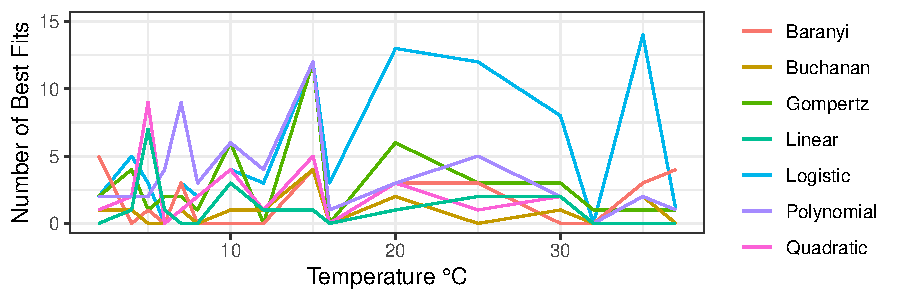
\includegraphics[width=13cm]
        {../results/AIC_temp_plot.pdf}}
        \caption{\label{fig:my-label} Number of best fits by temperature (AIC)}
      \end{figure}
      
      \begin{figure}[!htb]
        \center{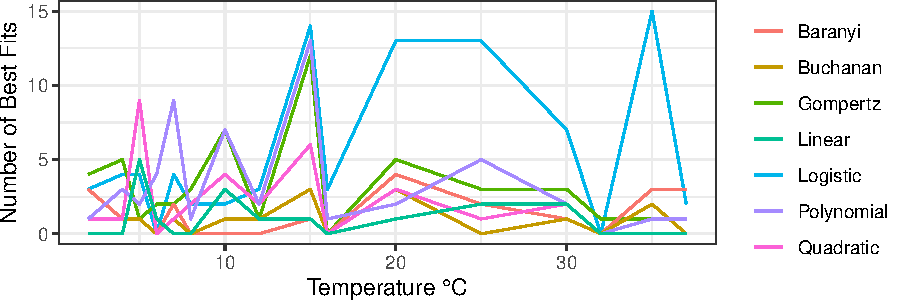
\includegraphics[width=13cm]
        {../results/BIC_temp_plot.pdf}}
        \caption{\label{fig:my-label} Number of best fits by temperature (BIC)}
      \end{figure}

When subset by temperature, the Logistic model showed best fits at higher temperatures for both AIC and BIC (Fig. 1 \& 2). Polynomial and Gompertz models exhibited a great number of best fits across low to mid temperature conditions. All other models showed no significant change in number of best fits across temperature conditions.

\begin{figure}
    \centering
    \begin{subfigure}[t]{0.45\textwidth}
        \centering
        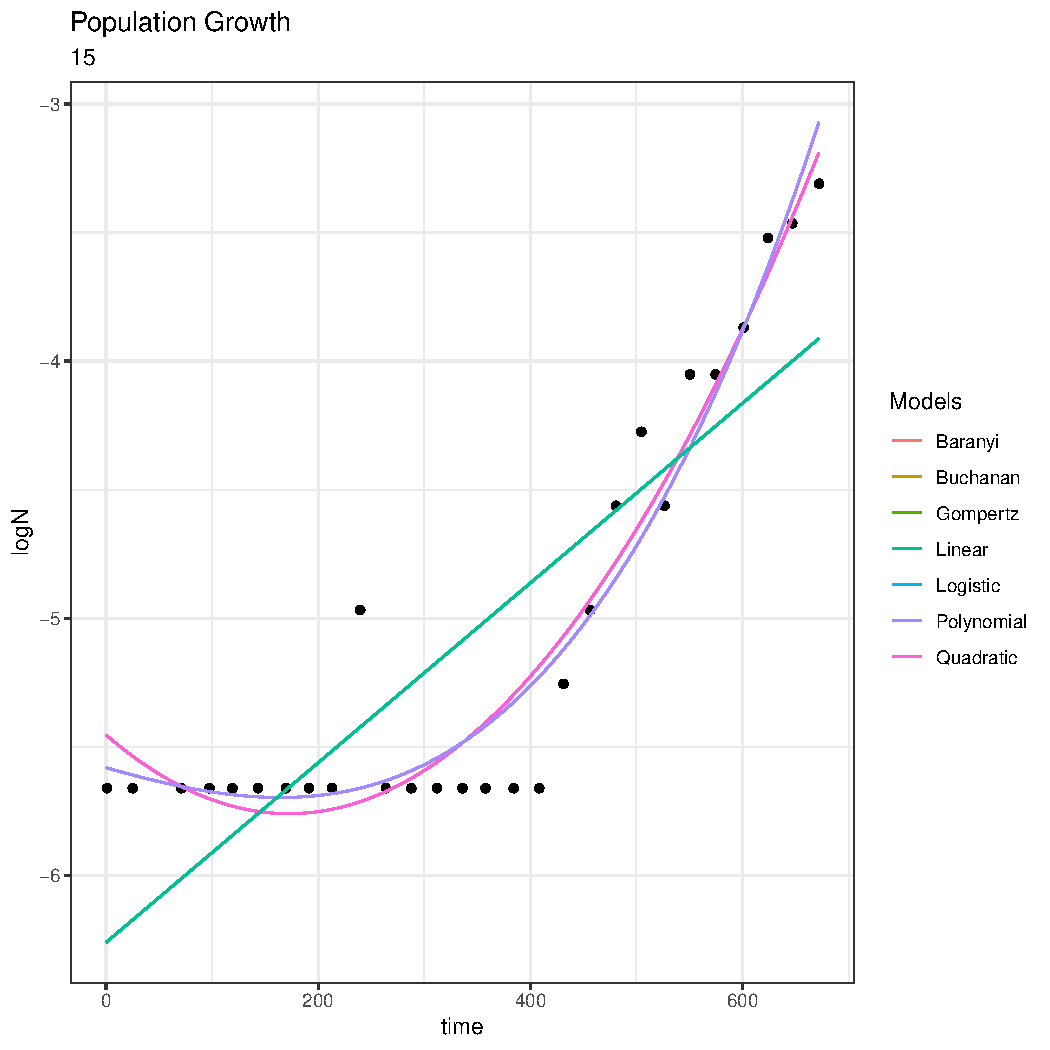
\includegraphics[width=\linewidth]{../results/plot_fits/plot_15.pdf} 
        \caption{Growth curve 15} \label{fig:timing1}
    \end{subfigure}
    \hfill
    \begin{subfigure}[t]{0.45\textwidth}
        \centering
        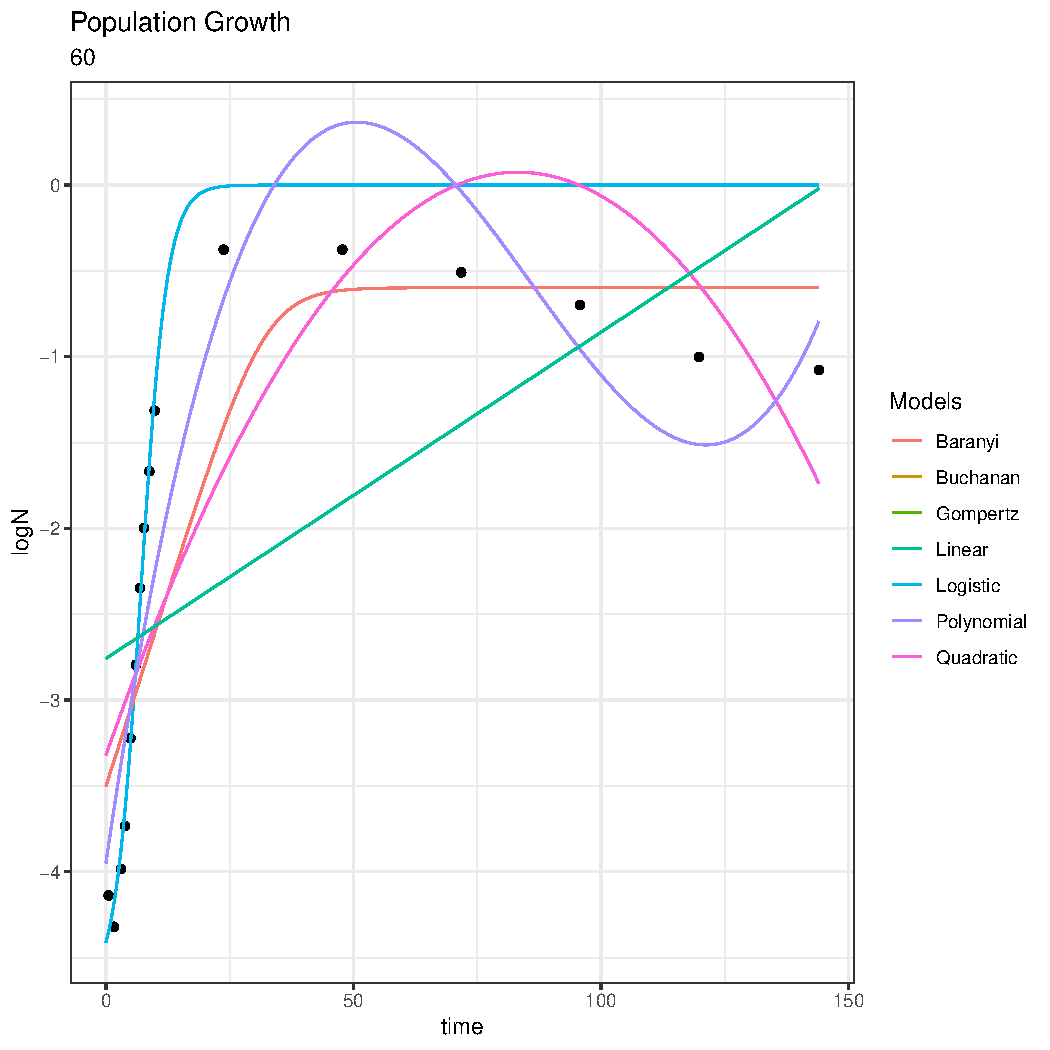
\includegraphics[width=\linewidth]{../results/plot_fits/plot_60.pdf} 
        \caption{Growth curve 60} \label{fig:timing2}
    \end{subfigure}

    \vspace{1cm}
    \begin{subfigure}[t]{0.8\textwidth}
    \centering
        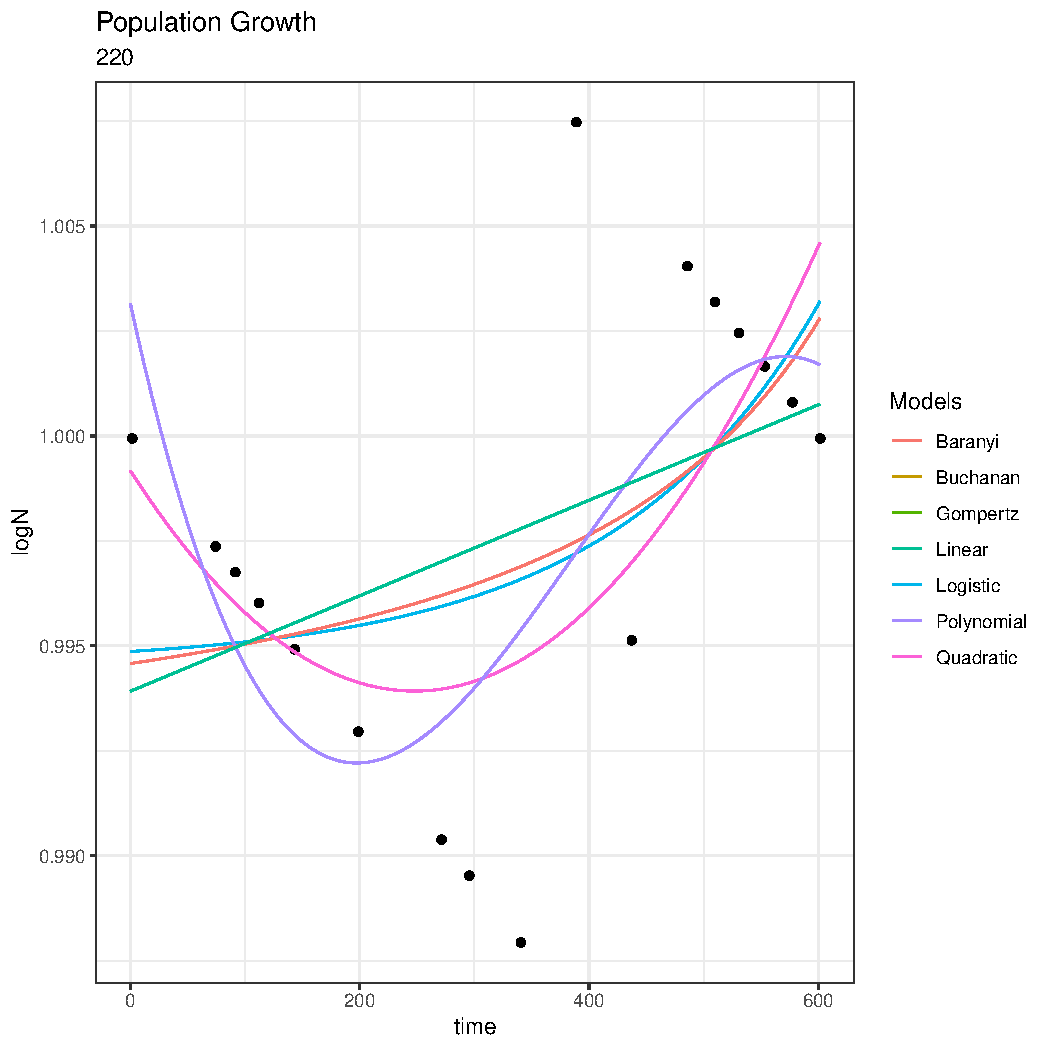
\includegraphics[width=0.8\linewidth]{../results/plot_fits/plot_220.pdf} 
        \caption{Growth curve 220} \label{fig:timing3}
    \end{subfigure}
    \caption{Example of poor visual fits}
\end{figure}

\section{Discussion}
In this report three statistical measures were applied to our model fits; $R^2$, AIC and BIC. An $R^2$ value indicates how closely the regression line is fit to the data or how much of the variation in the dataset's dependent variable is explained by the model. $R^2$ offers a good measure of fit but not of comparison between models as it does not take into account complexity of models. The $R^2$ statistic, therefore, prioritises parameter rich models, disregarding the principle of parsimony \cite{johnson2004model}. $R^2$ data included in Tab. 1 are present for contrasting with AIC and BIC methods only. $R^2$ is not used here when drawing comparisons between our competing models. AIC takes into account the sample size, residual sum of squares and number of parameters. AIC and BIC are structurally similar model selection criteria, however, the latter includes a sample size penalty term and favours simplicity \cite{johnson2004model}. The variation between AIC and BIC in this report is negligible as both produced similar results across the total data set. BIC did indicate Gompertz as the best fitting model for the \textit{Pseudomonas flurescens} group, where AIC found the same number of best fits between Polynomial, Logistic and Gompertz models for this species. Alternative model selection approaches include likeihood ratio and Bayesian tests, however, AIC and BIC are commonly preferred due to their grounding in Kullback–Leibler information theory \cite{johnson2004model}. \
      
\indent The Logistic model proved the best overall fit for the entire dataset, as per both AIC and BIC methods. The Logistic model was most successful under BIC selection, with 15 more best fits than AIC. This is due to BIC penalising additional model parameters where the Logistic model omitted time lag estimations. Less parameters produce a more stable solution as there is less inter-parameter correlation \cite{zwietering1990modeling}.\

  \indent The Polynomial model showed the second greatest number of best fits. However, for an equation to be considered a model there must be underlying physiological relationships \cite{baranyi1995mathematics}. The Polynomial, Quadratic and Linear models used in this report are purely phenomenological, with no opportunity for mechanistic interpretation. Therefore, despite the successful fitting of the Polynomial model, it is not useful for the purpose of predicting microbial population growth in any meaningful or applicable way. \
  
  \indent Previous investigations have found better fits with the Gompertz model, as opposed to the Logistic model, with little success fitting Linear and Quadratic models \cite{zwietering1990modeling}. The contrast with our own findings may be due to species differences, experimental error or design. A greater number of data points per dataset appears to reduce the importance of parameter numbers in model fitting and this may account for the discrepancy in results \cite{zwietering1990modeling}. Gompertz has also been shown to be more successful at fitting bacterial growth curves than the Baranyi model, which is in keeping with our findings \cite{buchanan1997simple}. \
  
\indent The poor performance of the popular Baranyi model may be due to its conceptual problems. The model assumes a universal relationship between lag time and maximum growth rate \cite{peleg2011microbial}. Previous studies have found that the parameters have an inverse relationship, but cannot be used to predict one another as the shape of the growth curve is determined by the state of the system, not the relationship between lag and growth \cite{brown2007two}.\ 

\indent Polynomial, Quadratic and Linear models showed the highest rate of successful fitting (99-100\%). Visual inspection indicated many of these 'successful' fits were poor (Fig. 3). The success of these models is due to their fitting using the ordinary least squares method, in contrast to the other four models that are fit using the Levenberg-Marquardt nonlinear least squares method that uses convergence.  \

\indent The Logistic model showed greater success when applied to datasets with higher temperature treatments. It might be suggested that as temperatures increase so growth rate increases and lag time to initiate the appropriate biochemical reactions for division decreases. Where the Logistic model lacks a time lag parameter, unlike the Gompertz, Baranyi and Buchanan models, it may be a better fit to datasets where higher temperatures have rendered the initial lag phase redundant. Rising temperatures eventually lead to peak growth followed by 'thermal inactivation' \cite{peleg2011microbial}. The maximum temperature condition for our datasets was 37\degree C and there was some evidence of thermal inactivation in the poor visual fits (Fig. 3). This shows the need for a model that is thermally sensitive and addresses mortality rate. \

\indent When grouped by species the Logistic model continued to be the most successful in seven out of eleven groups. Although the Quadratic model was the most successful for two groups, in contrast to its overall poor performance. The success of models differs between species due to the relative influence of system characteristics \cite{zwietering1990modeling}. 

\indent Whilst all the models included in this report show at least some degree of success, there are general problems that need to be addressed. Primarily, none of the four more mechanistic models address cell mortality. The lag and stationary phases may represent a lack of cell division or equality between division and mortality rate. Growth rate change may be a function of division or death, we have no way of knowing. It is difficult then, to consider these models particularly mechanistically informative. What can be inferred physiologically about life, without considering death? Moreover, if empirical sigmoidal equations such as the Gompertz model, differential rate equations, such as the Logistic model, and multiple linear regressions such as the Polynomial model, can all be successfully fit to the same dataset, it is diffcult to infer mechanistic meaning from the parameters \cite{peleg2011microbial}.\
      
  
  





\section{Conclusion}
Across all data sets, in total and subdivided by species, the Logistic model most frequently achieved best fits. This result supports the popularity of this model for fitting bacterial growth curves. As none of these models can be defined as truly mechanistically informative, it is sensible to select the simplest and the best fitting. The Logistic model appears to fulfil these requirements and is, therefore, the most appropriate model for our dataset \cite{peleg2011microbial}. The Logistic model in this instance showed not only the greatest number of best fits, but it was simpler than Gompertz, Baranyi and Buchanan models, requiring only three input parameters, instead of four.\

\indent One limitation of this report is the variety of datasets used. The particular methods for collecting these data, likely vary between investigations. In order to further assess how well different mathematical models fit bacterial population growth curves it would be desirable to conduct a single, large scale empirical investigation. This would control for variation across methods. \

\indent Here, the Logistic model was significantly better at fitting the data than any other model, however, the benefits of model comparison are such that if two or more models had show similar success, model averages could be obtained to produce robust parameter estimates (\cite{johnson2004model}. It might then be advisable to combine the Logistic and Gompertz models to the find the most robust parameters for bacterial growth estimation. \

\indent The growth curves modelled here are representative of a suite of underlying physiological processes. However, there is not enough information within the curves to glean mechanistic interpretation. Moreover, the value of parameters used in constructing our models are dependent on experimental error, design and model bias \cite{grijspeerdt1999estimating}. In order to define useful parameters and understand the mechanisms involved, specific experiments must be conducted to assess the underlying physiological processes and their relationship with the characteristics of the system \cite{peleg2011microbial}. \

\indent In order to gain more mechanistic insight into bacterial growth patterns, models must be developed that define growth rate as a function of system characteristics, such as temperature, pH and medium. Developing such models sacrifices the generality that makes those discussed in this paper so widely applied. Explicit experimentation may help in defining the way system characteristics not only affect bacterial growth patterns, but also the physiological implications of those interacting characteristics. It appears that, for now, we do indeed make sacrifices in the search for generality, realism and precision \cite{levins1966strategy}.\



\bibliographystyle{plain}
\bibliography{bibliography}

\section{Appendix}

\begin{table}[!htbp]
\catcode`"=9
\centering
\caption{AIC Species Best Fits}
\csvautotabular{../results/species_stats_AIC.csv}
\end{table}


\begin{table}[!htbp]
\catcode`"=9
\centering
\caption{BIC Species Best Fits}
\csvautotabular{../results/species_stats_BIC.csv}
\end{table}


\begin{table}[!htbp]
\catcode`"=9
\centering
\caption{AIC Temperature Best Fits}
\csvautotabular{../results/temp_stats_AIC.csv}
\end{table}


\begin{table}[!htbp]
\catcode`"=9
\centering
\caption{BIC Temperature Best Fits}
\csvautotabular{../results/temp_stats_BIC.csv}
\end{table}


\end{document}
